\chapter{Write and run your first world}

This chapter steps you through the writing and running of your first world. In the process it explains \textsc{Becca}'s structure at a high level.

\section{What is a world?}

A \textsc{Becca} {\em agent} is a thing that chooses actions. In order for those actions to have any effect, they must be coupled to a {\em world}, an external environment that the agent can interact with. The agent--world configuration that \textsc{Becca} uses is shown in Figure~\ref{agent_world}. It is the canonical statement of the reinforcement learning problem: a reinforcement learning agent tries to choose actions so as to maximize the reward it receives.~\cite{sutton98} 

\begin{figure}
\centering
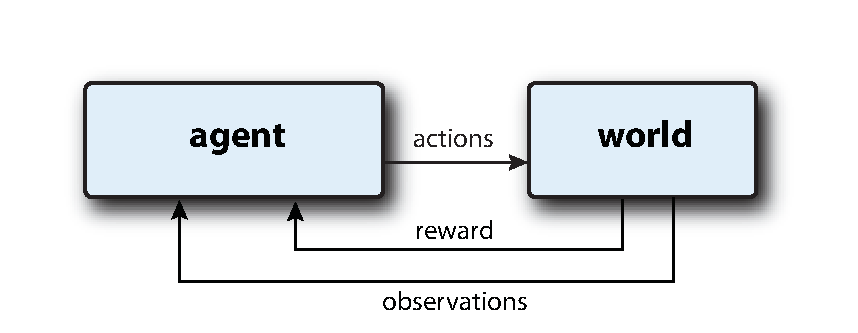
\includegraphics[height=5.0cm]{figs/agent_world.eps}
\caption{The agent-world coupling in \textsc{Becca}. The agent selects actions to execute on the world, which in turn provides observations and reward feedback.}
\label{agent_world}
\end{figure}

The architecture is modular. You can develop and run your own worlds without having to know very much about how the \textsc{Becca} agent works. The only constraints \textsc{Becca} imposes on worlds are:

\begin{itemize}
\item{A world must read in a fixed number of actions at each time step. This number is chosen by and defined in the world.}
\item{A world must provide a fixed number of sensory observations at each time step. This number is also chosen by and defined in the world.}
\item{A world must provide a scalar reward value at each time step.}
\item{All actions and observations are real valued, equal to 0, 1, or something in between.}
\item{The reward signal is real valued, equal to -1, 1, or something in between.}
\end{itemize}

Strictly speaking, \textsc{Becca} allows for two classes of observations, {\em sensors} and {\em primitives}. The only difference between the two is that the agent has to build sensors into features before it can use them, whereas it can use primitives as features immediately. Typically, observations that are likely to need some refining before they become useful (such as sets of pixel values) are passed in as sensors, and observations that are more immediately useful (such as a contact sensor) are passed in as primitives. 

\section{How do I make a {\em hello} world?}

The quick and dirty way to get started making your own world is to copy an existing one and modify it. This is especially effective if there already exists something roughly similar to what you want. That's the approach we'll use to make a hello world.

\begin{enumerate}
\item{Save \texttt{worlds/grid\_1D.py} as \texttt{worlds/hello.py}}
\item{Replace the body of \texttt{step()} with this:
\begin{verbatim}
self.timestep += 1 
print self.timestep, ' hellos!'

sensors = np.zeros(self.num_sensors)
primitives = np.zeros(self.num_primitives)
reward = 0
return sensors, primitives, reward
\end{verbatim}
and save the changes.
}
\item{Add the line 
\begin{verbatim}
from worlds.hello import World
\end{verbatim}
to \texttt{tester.py}. Make sure all the other lines beginning with \texttt{from worlds}...  are commented out.
}
\item{Run \texttt{tester.py}}
\end{enumerate}


\section{What do I need to implement in my world?}

\texttt{hello.py} runs because it meets a few basic requirements. This section lists them and describes the mechanics of a \textsc{Becca} world.

Any world needs to have at least these three publicly accessible member variables,

\begin{itemize}
\item{\texttt{num\_sensors}}
\item{\texttt{num\_primitives}}
\item{\texttt{num\_actions}}
\end{itemize}

these three methods,

\begin{itemize}
\item{\texttt{step()}}
\item{\texttt{is\_alive()}}
\item{\texttt{set\_agent\_parameters()}}
\end{itemize}

and perhaps two optional methods,

\begin{itemize}
\item{\texttt{is\_time\_to\_display()}}
\item{\texttt{vizualize\_feature\_set()}}
\end{itemize}

each of which are all described in more detail below.

\subsection{\texttt{num\_sensors}}
Specifies the number elements in the array of sensor information that is passed to the agent at each time step.

\subsection{\texttt{num\_primitives}}
Specifies the number elements in the array of feature primitives that is passed to the agent at each time step.

\subsection{\texttt{num\_actions}}
Specifies the number elements in the array of actions that it expects to receive from the agent at each time step. Together, these three variables define the interface between the agent and the world. They may be different for each world, but they must remain constant within a single world. \footnote{In this version of \textsc{Becca}, each of these variables must be at least 1. \textsc{Becca} doesn't yet know how to handle empty sensory or primitive arrays. Worlds that have no sensors or primitives can pass a single zero value at every time step to achieve this.}

\subsection{\texttt{step()}}
Advances the world by one time step. This is single most important method in a world. It defines how the world will respond to the agent. It accepts an array of actions and returns an array of sensors, an array of primitives, and a reward value. \textsc{Becca} places no constraints on the complexity or the execution time of the \texttt{step()} method. It can incrementally advance a simulation, pass and receive network packets, or provide an interface to physical robot. The agent will wait until \texttt{step()} finishes and returns its observation and reward information before advancing to the next time step.

\subsection{\texttt{is\_alive()}}
Informs the executing loop when to stop. The top level execution loop (as implemented in \texttt{benchmark.py} and \texttt{tester.py} continues to run \textsc{Becca} through its agent-world-agent cycle until \texttt{is\_alive()} returns false.

\subsection{\texttt{set\_agent\_parameters()}}
Sets the the agent's internal parameters to values specific to the world. \textsc{Becca} has a quite a few constants that affect its operation, in the neighborhood of 20 at last count. Most of these are set to values that seem to work for all worlds in the benchmark battery. But for development and troubleshooting, it has proven useful to be able to adjust some of \textsc{Becca}'s parameters manually. It is my hope that, in time, a single set of parameters will prove generally useful across a broad set of tasks. In the meantime this method provides a mechanism for world-specific knob-twiddling.

\subsection{\texttt{is\_time\_to\_display()}}
Informs the executing loop when to display the feature set by returning \texttt{True}. This is for visualization purposes only and doesn't help \textsc{Becca} learn in any way. This method is optional. If it doesn't exist, the execution loop just moves on.

\subsection{\texttt{vizualize\_feature\_set()}}
Displays the feature set when \texttt{is\_time\_to\_display()} returns \texttt{True}. The feature set is expressed in terms of sensors, primitives, and actions by the agent. This method takes those feature representations and interprets them for the user in terms of what it knows about how those signals. For instance, if the sensors correspond to pixel values from a camera, this method would render the sensor component of each feature as an image. The agent has no information about where its sensor and primitive arrays came from or about what its actions do in the world. This method lets the world give a world-specific interpretation of those values to the user.

Worlds of course may have any number of other member variables and methods for internal use. Others that have proven useful in the benchmark battery worlds include \texttt{calculate\_reward()} and \texttt{display()}.

\section{What is \texttt{base\_world.py}?}
``Wait a second," you say. ``My \texttt{hello.py} didn't have an \texttt{is\_alive()}, but you said it needed one. What's up with that?"

These two lines from the beginning of the module help to solve that mystery:
\begin{verbatim}
from .base_world import World as BaseWorld
class World(BaseWorld):
\end{verbatim}

\texttt{hello.py} is actually a subclass of \texttt{base\_world.py},\footnote{If terms like {\em class}, {\em subclass}, {\em inheritance}, and {\em override} aren't familiar to you in this context, I'd highly recommend doing some quick reading on object-oriented (OO) programming. The concepts aren't that tricky, but they are extremely useful when discussing OO software, like \textsc{Becca}.} which defines a generic \texttt{is\_alive()}. It also defines a generic \texttt{set\_agent\_parameters()} and \texttt{step()}, as well as default values for  \texttt{num\_sensors}, \texttt{num\_primitives}, and \texttt{num\_actions}. When you subclass it to create a new world you, only need to override those methods and variables that you want to change.


\section{How do I run my world?}
\texttt{tester.py} is the vehicle for coupling a new world with a \textsc{Becca} agent and running them. You've already added your hello world to \texttt{tester.py} and run it. This section gives a line-by-line overview of the rest of the module and what it does. This will help make clear a few of the finer points of running a world.

\begin{enumerate}
\item
Import the relevant modules. In particular import a \texttt{World} class from a module containing one.
\begin{verbatim}
import numpy as np
from agent.agent import Agent
from agent import viz_utils
from worlds.hello import World
\end{verbatim}

\item
Define the \texttt{main} method and initialize some objects. When initializing the \texttt{agent}, there are two optional variables, \texttt{MAX\_NUM\_FEATURES} and \texttt{agent\_name}.  \texttt{MAX\_NUM\_FEATURES} provides an upper limit on the number of features that the agent can create and can be set appropriately to prevent \textsc{Becca} from using up all your RAM. \texttt{agent\_name} is a text string used to identify a specific agent and is useful if you are planning to save the agent or restore it from a previously saved agent. Note that if you do this, the world used in both cases must have the same number of sensors, primitives, and actions.
\begin{verbatim}
def main():
    
    world = World()
    
    agent_name = "test";
    MAX_NUM_FEATURES = 3000
    agent = Agent(world.num_sensors, 
                  world.num_primitives, 
                  world.num_actions, 
                  MAX_NUM_FEATURES, 
                  agent_name)

\end{verbatim}

\item
Restore the agent to a previously saved agent, if desired.
\begin{verbatim}
    #agent = agent.restore()
\end{verbatim}
    
\item
Modify the agent's parameters according to the requirements of this particular world. Initialize actions such that the first set of commands to the world is always zeros.
\begin{verbatim}
    world.set_agent_parameters(agent)
    actions = np.zeros(world.num_actions)
\end{verbatim}

\item
Begin the execution loop. Couple the output of the world into the input of the agent and vice versa.
\begin{verbatim}    
    while(world.is_alive()):
        sensors, primitives, reward = world.step(actions)
        actions = agent.step(sensors, primitives, reward)
\end{verbatim}

\item
If the necessary methods exist, and if they dictate, display the feature set to the user.        
\begin{verbatim}    
    try:
        if world.is_time_to_display():
            world.vizualize_feature_set(
                viz_utils.reduce_feature_set(
                agent.grouper), 
                save_eps=True)
            viz_utils.force_redraw()
    except AttributeError:
        pass
\end{verbatim}

\item
After the world has completed its lifetime, give a final report of the agent's performance.    
\begin{verbatim}    
    agent.report_performance()
    agent.show_reward_history()
    
    return
\end{verbatim}

\item
And finally, run \texttt{main()}    
\begin{verbatim}    
if __name__ == '__main__':
    main()
\end{verbatim}

\end{enumerate}

% TODO: flesh this out
%\section{Are there any tricks for making a world so that \textsc{Becca} can learn it?}
% binary-style inputs
% make sure Becca gets enough information--could a human solve the task?
% primitives--high-level sensors
% actions--high level vs. low level
